\documentclass[12pt]{article}
% chktex-file 3
% chktex-file 13
% chktex-file 8
% chktex-file 18
% chktex-file 12
\usepackage[utf8]{inputenc}
\usepackage[T1]{fontenc}
\usepackage{graphicx}
\usepackage[export]{adjustbox}
\graphicspath{ {./images/} }
\usepackage{amsmath}
\usepackage{amsfonts}
\usepackage{amssymb}
\usepackage[version=4]{mhchem}
\usepackage{stmaryrd}
\usepackage{geometry}
\geometry{margin=1in}
\usepackage[hidelinks]{hyperref}

\title{RBE 4540 --- Group Assignment: Top Surface Grasping}
\author{Brent Weiffenbach, Isabella Rosenstein, Evan Carmody}
\date{\today}

\begin{document}
\maketitle

The goal of this project is to identfy the top surface of any number of objects, and estimate the shape of the surface as a 2D polygon. The polygon will be used to plan a grasp with the best quality metrics to pick up the object.

\begin{center}
	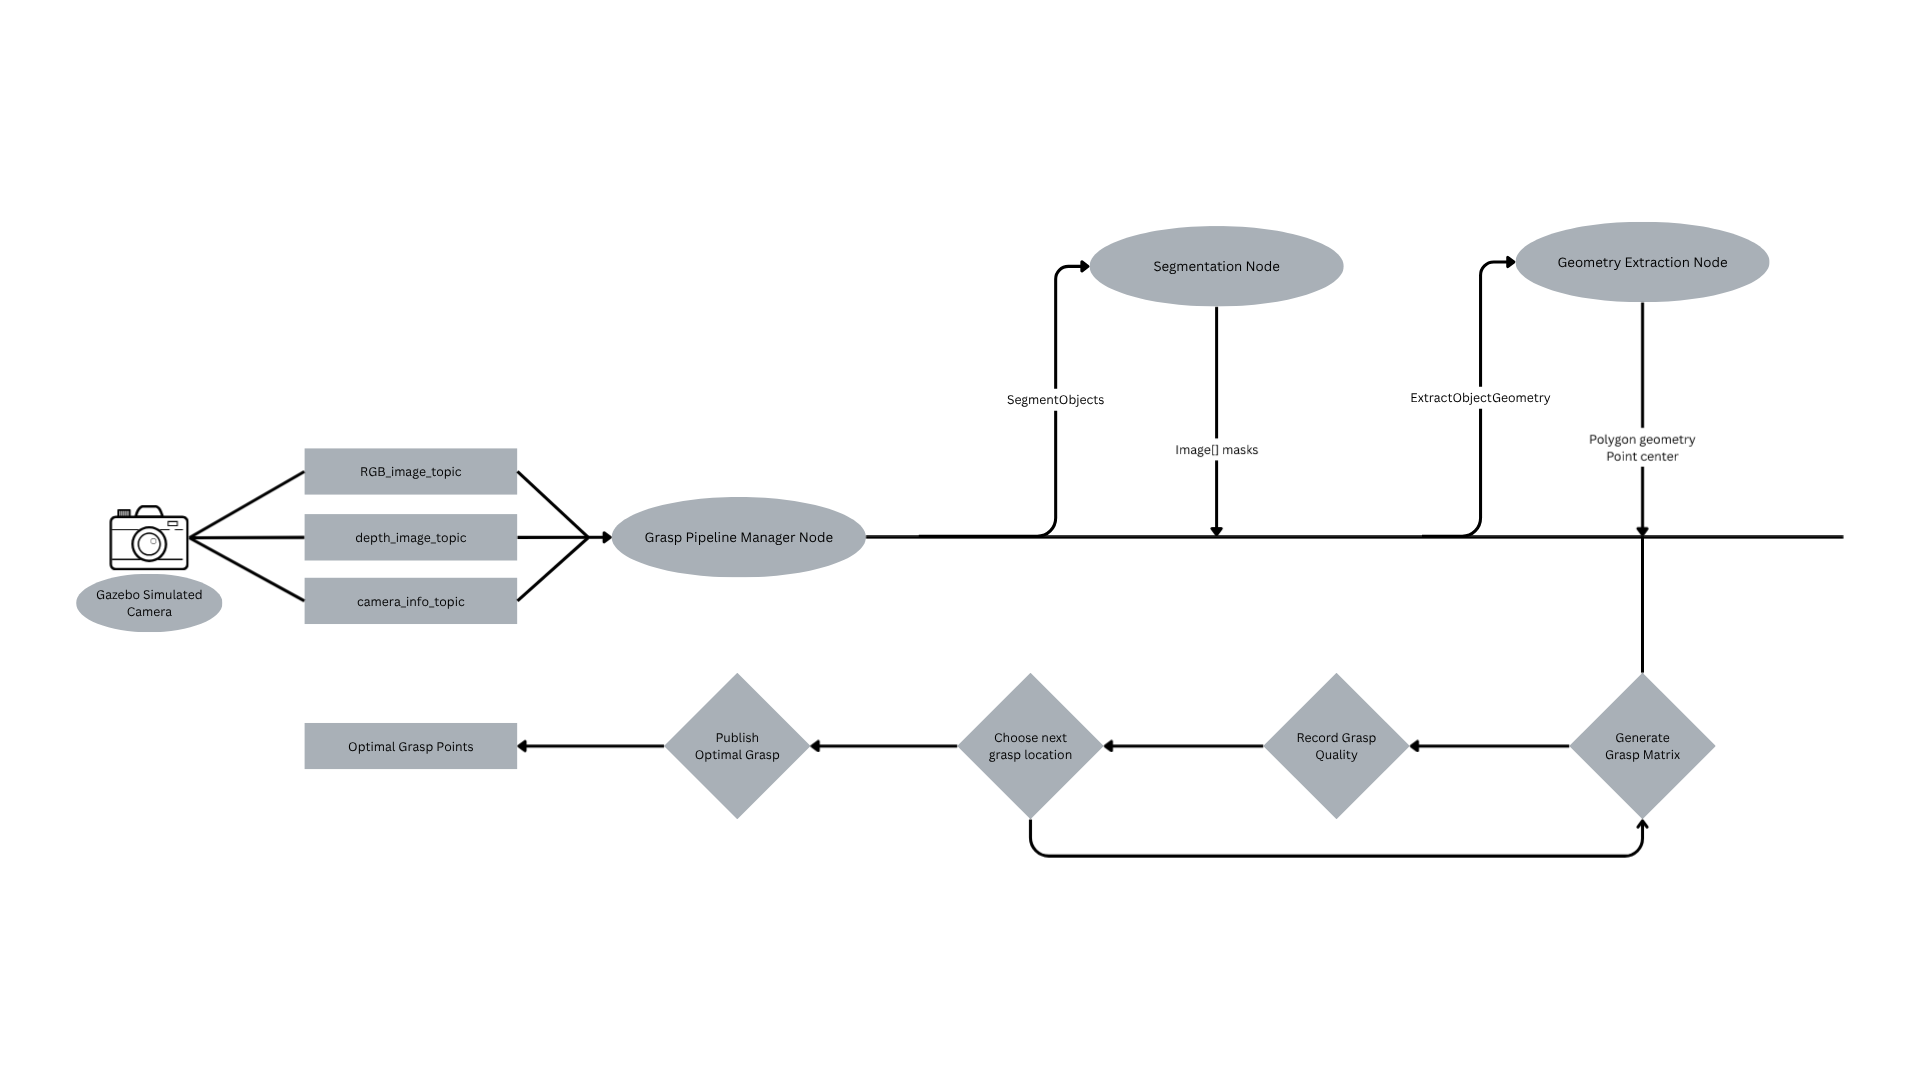
\includegraphics[width=0.8\textwidth]{TopGraspingArchiteture.png}
\end{center}

\vspace{0.3cm}

\textbf{Step 1: Enviornment Setup}

This project contains 5 ROS packages. A launch file at the root of the \textbf{TopSurfaceGrasping} folder which is not part of a specific ROS2 package launches all the necessary nodes. 

First we open a gazebo world with a table, 2 coke cans, banana, and mustard bottle in it. Then we spawn in the camera above the table looking at an angle towards the objects. To keep a global world frame we can use to identify what the `top' of surfaces is, we use a static transform publisher to publish a transform from the camera frame to the world frame.

\begin{center}
	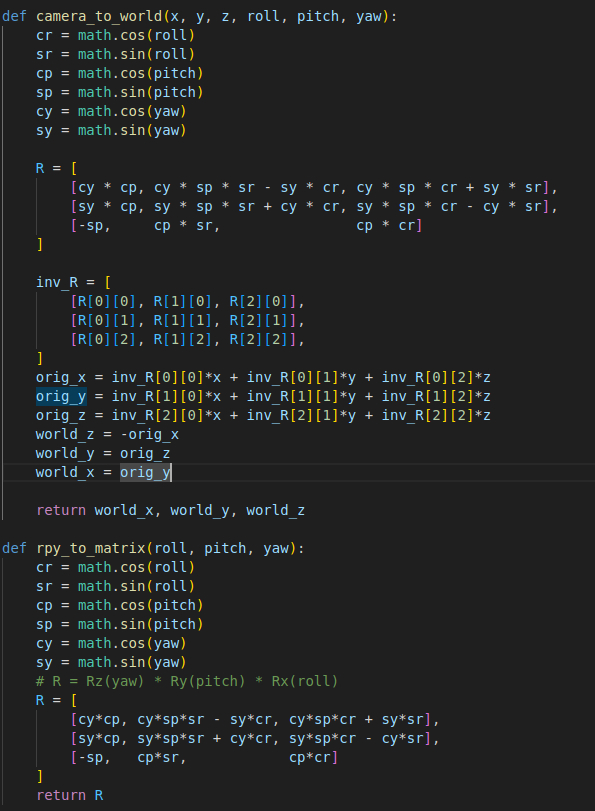
\includegraphics[width=0.8\textwidth]{launchhelpers.png}
\end{center}

We use these helper functions in the launch file to convert from camera coordinates to world coordinates, and keep the world frame aligned with the table surface.

With that we have a gazebo world with objects in it, and a camera looking at the objects, where the camera publishes RGB and depth information to ROS topics.

Finally, we have a grasp pipeline manager node which will manage the flow of data and publish debug information to topics we can view in rviz. The pipeline manager will call services on the segmentation and geometry extraction nodes.

\begin{center}
	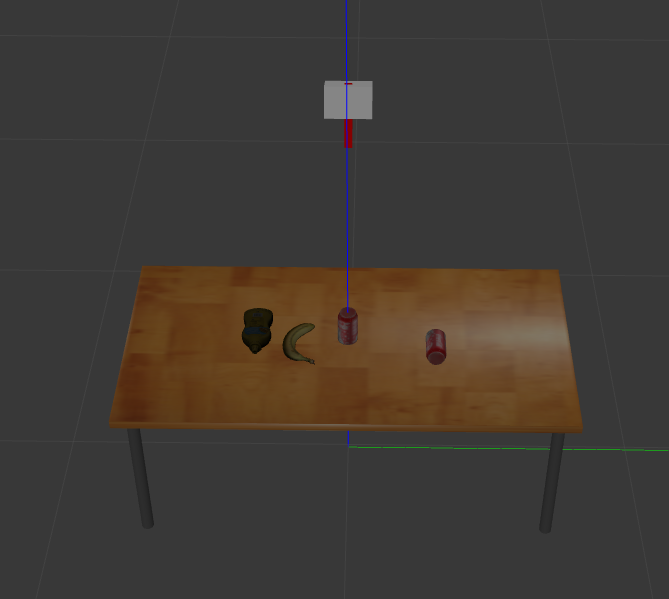
\includegraphics[width=0.8\textwidth]{gazebo.png}
\end{center}

\textbf{Step 2: Image Processing}

Given an RGB image, we need to detect the objects in the image, and create a mask for each object. The \texttt{SegmentationNode} has a service \texttt{segment\_objects} which receives an RGB image from the pipeline manager, and returns a list of masks for each detected object. It processes the image by masking out background regions like the table and sky to isolate the objects. Then contours are found in the masked image, and if the area is large enough, a mask is created for the object. 

Code for getting the masks:

\begin{center}
	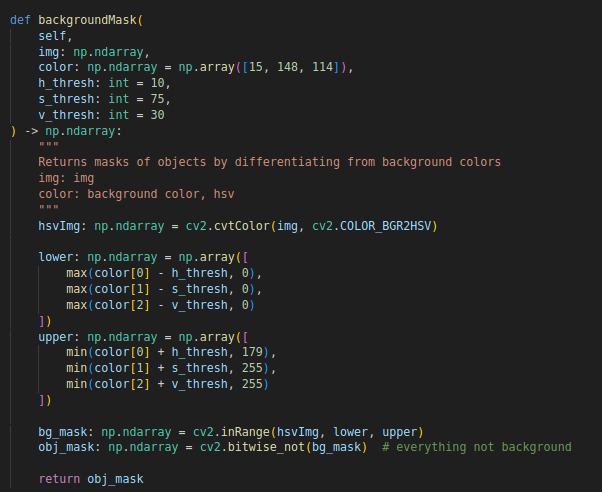
\includegraphics[width=0.8\textwidth]{vision/backgroudmask.png}
\end{center}

\begin{center}
	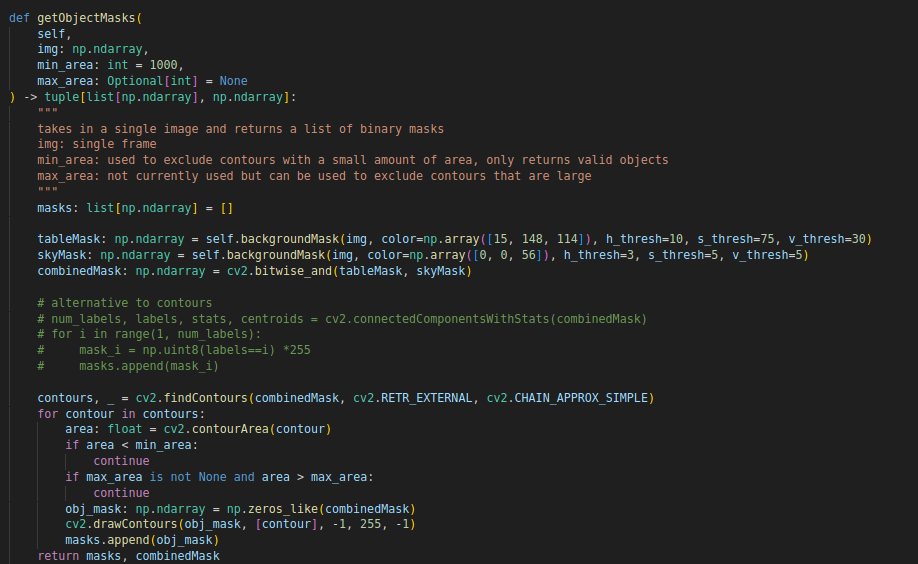
\includegraphics[width=0.8\textwidth]{vision/getobjectmasks.png}
\end{center}

\begin{center}
	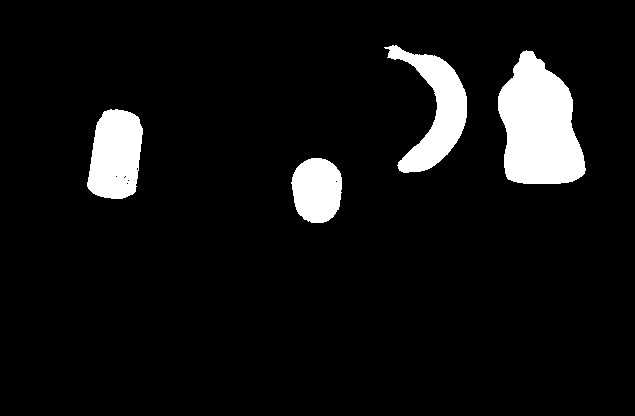
\includegraphics[width=0.8\textwidth]{masks.png}
\end{center}

\textbf{Step 3: Geometry Extraction}

The \texttt{GeometryExtractionNode} has a service \texttt{extract\_object\_geometry} which receives a list of masks and a point cloud and returns a polygon representing the top surface and the center of mass projected onto the top surface. The node first masks the point cloud to isolate only relevant points of the object, then selects all the points with the minimum y-value (world coordinate system makes this the top surface), and projects these points into a 2D plane. Then using OpenCV contour detection, the top surface polygon is found. The center of mass is calculated by averaging the x and z coordinates of the top surface point cloud points, and using the minimum y-value for the y coordinate. The code callback for the service is too long to include in the report, but the code can be found in the submission files.

\begin{center}
	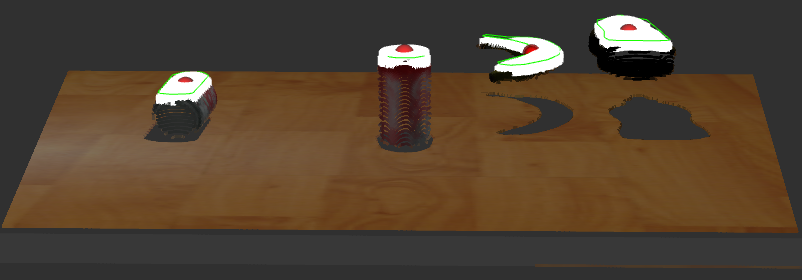
\includegraphics[width=0.8\textwidth]{toppoints.png}
\end{center}

\textbf{Step 4: Finding a Grasp}

Once we have a polygon and center of mass, we can preform similar steps to previous homework assignments to find a grasp. We generate a list of grasp candiates on the object, and evaluate each candidate using grasp quality metrics. We find the minimum singular value, isotropy, and volume of ellipsoid metrics for each candidate, and select the candidate with the best metrics (if it has 2 metrics that are the best). Then these contact points can be visualized as markers in rviz.

\begin{center}
	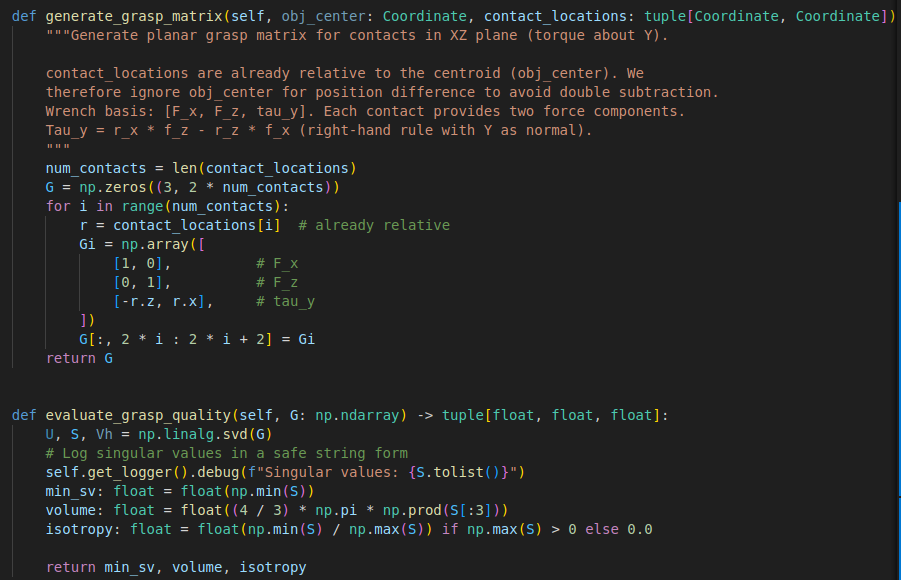
\includegraphics[width=0.8\textwidth]{graspmatrixcode.png}
\end{center}

Code for grasp candidates:
\begin{center}
	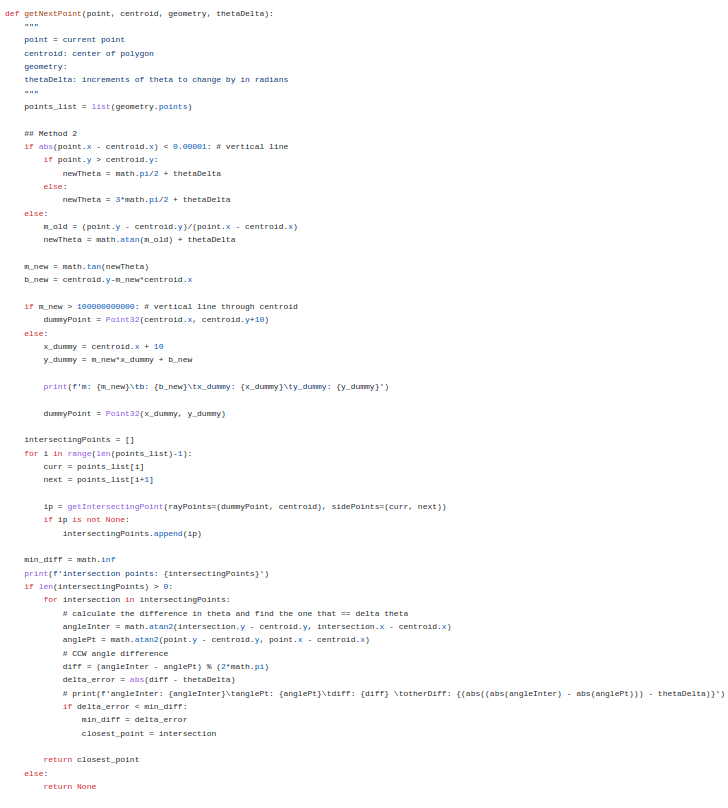
\includegraphics[width=0.8\textwidth]{get_next.png}
\end{center}

\begin{center}
	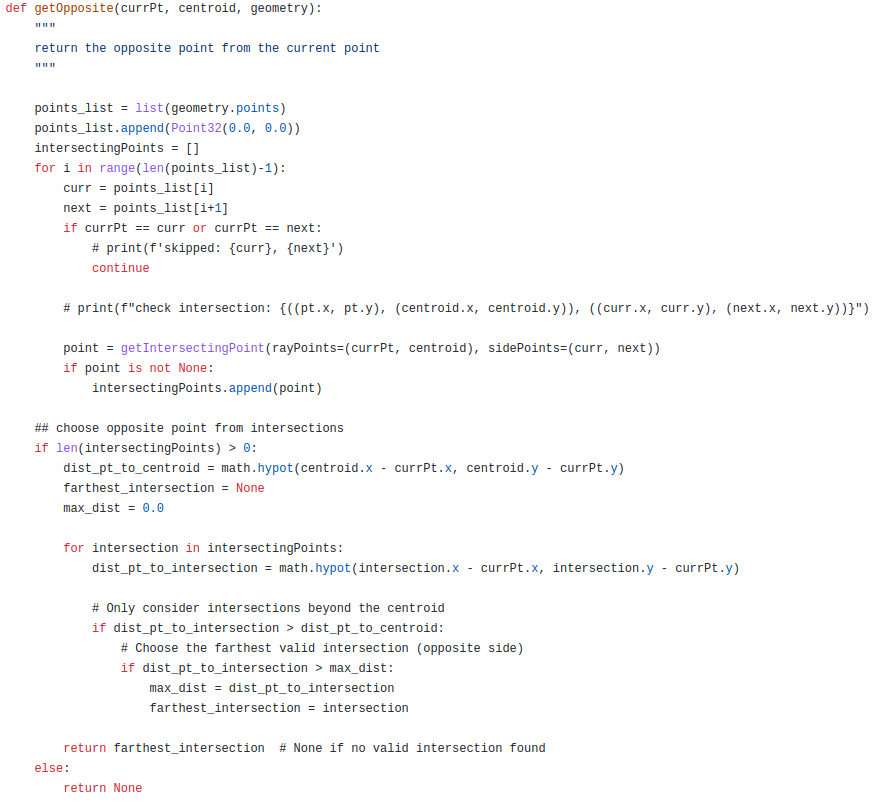
\includegraphics[width=0.8\textwidth]{get_opposite.png}
\end{center}

\begin{center}
	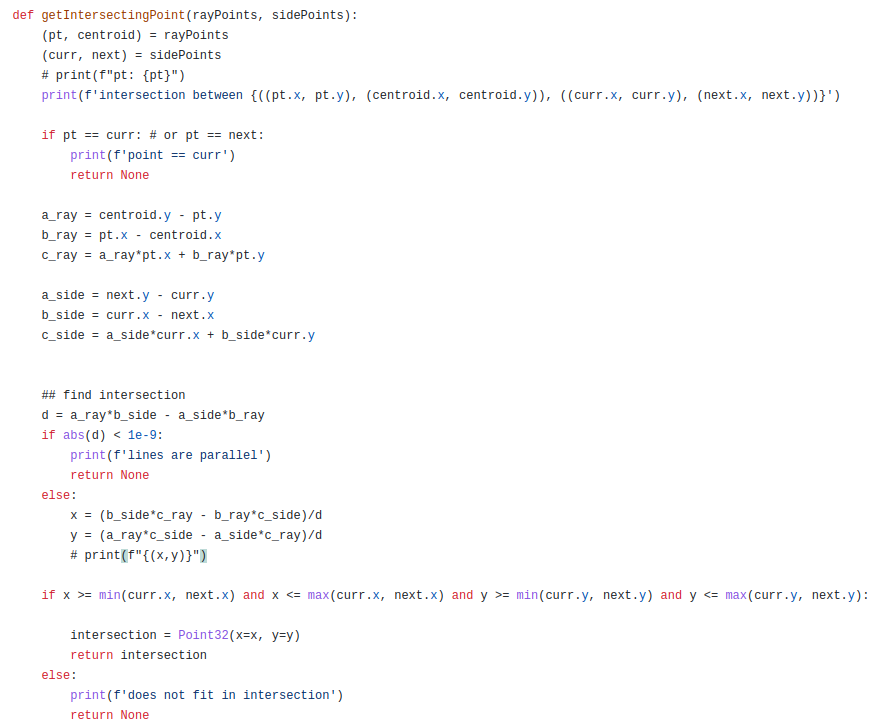
\includegraphics[width=0.8\textwidth]{getintersect.png}
\end{center}

\begin{center}
	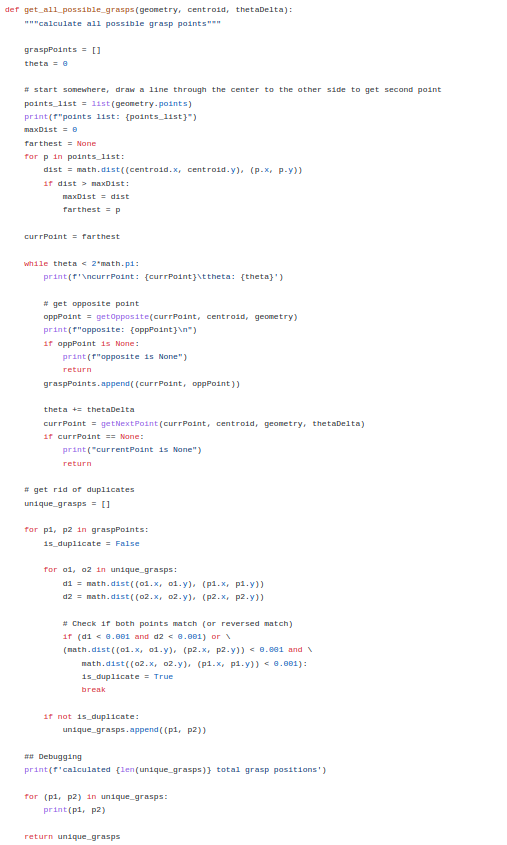
\includegraphics[width=0.8\textwidth]{allpossiblegrasps.png}
\end{center}

\section*{Discussion}

\begin{center}
	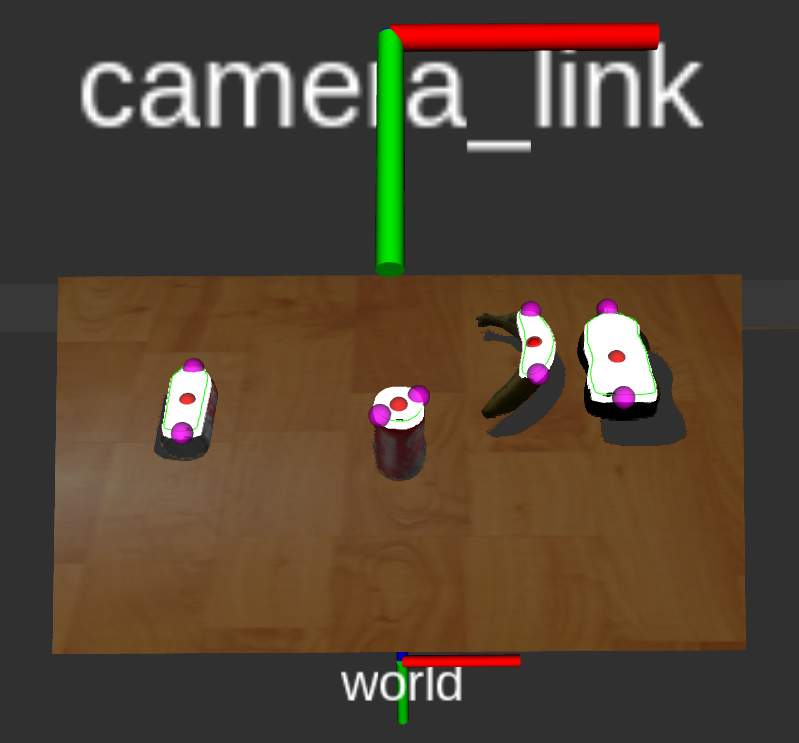
\includegraphics[width=0.8\textwidth]{final_grasps.png}
\end{center}

We had resulting grasps with the following metrics:

\begin{itemize}
	\item \textbf{Object 1 (Standing Coke Can):} \\
	Best grasp with $\min\_sv=0.0428$, $volume=0.3588$, $isotropy=0.0303$
	\item \textbf{Object 2 (Lying Down Coke Can):} \\
	Best grasp with $\min\_sv=0.0870$, $volume=0.7286$, $isotropy=0.0615$
	\item \textbf{Object 3 (Mustard Bottle):} \\
	Best grasp with $\min\_sv=0.1209$, $volume=1.0130$, $isotropy=0.0855$
	\item \textbf{Object 4 (Banana):} \\
	Best grasp with $\min\_sv=0.0892$, $volume=0.7476$, $isotropy=0.0631$
\end{itemize}

As seen in the images, the grasps are reasonably placed and could sufficently pick up the objects. Our best grasp was on the mustard bottle, which is the object with the largest top surface area. The grasps on the two coke cans are also good, with the grasp on the lying down can being better than the standing can. The grasp on the banana is the worst, which makes sense as the top surface is very small and curved. We also are modeling the grasps as hard contacts, which could result in these grasps not being the exact ideal grasps a human would use. 

\end{document}